\scanpage{53}
\mspage{\handwritten{21}\,\raisebox{.5ex}{\begin{tikzpicture}[x=1cm,y=1cm,baseline=0pt]\draw[line width=.6pt] (0,-.02)--(.015,.025)--(.04,.04);\end{tikzpicture}}}
% archive sheet number: 52

$G=\underset{\handwritten{\longleftarrow}}{\lim}G_i$ (EGA IV 8.2 3). \deleted{The fact that} the transition morphisms are faithful-\linebreak 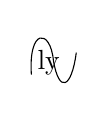
\begin{tikzpicture}[x=1cm,y=1cm,baseline=(n.base)]\node (n) at (0,0) {ly};\draw (-.22,-.16) .. controls (-.26,.43) and (.02,.43) .. (.06,.02) .. controls (.13,-.4) and (.29,-.34) .. (.35,.12);\end{tikzpicture} flat by the following lemma:
% A handwritten transposition mark joins the n and e of the line-end continuation.


\uline{Lemma \handwritten{11.14}.- Let $k$ be a field, $G$ and $H$ two affine $k$-groups of finite type, $u:G\handwritten{\longrightarrow}H$} a \uline{morphism of $k$-groups, and $u^{\unsure{o|0|\circ}}:B\handwritten{\longrightarrow}A$ the corresponding homomorphism of $k$-algebras .} For \uline{$u$ to be faithfully flat, it is necessary and sufficient that $u^{\unsure{o|0|\circ}}$ be injective.}

the condition is obviously necessary (EGA IV 2.2.3 and $\unsure{0|O}_{\mathrm{IV}}$ 6.6.1). Let us show that it is sufficient. Set $K=\operatorname{Ker}u$. Then $G/K$ is a $k$-group\inserted{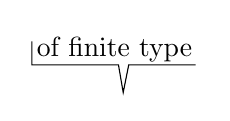
\begin{tikzpicture}[x=1cm,y=1cm,baseline=(n.base)]\node (n) at (0,0) {of finite type};\draw (-1.05,.1)--(-1.05,-.2)--(.05,-.2)--(.11,-.55)--(.18,-.2)--(1.03,-.2);\end{tikzpicture}} (\deleted{Exposition} $\mathrm{VI}_A$ 5.2), and $u$ factors as $G\mathrel{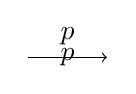
\begin{tikzpicture}[x=1cm,y=1cm,baseline=-.5ex]\draw[->] (0,0)--(1,0);\node[inner sep=0pt] at (.5,0) {$\deleted{p}$};\node[inner sep=0pt,above] at (.5,.15) {$\inserted{p}$};\end{tikzpicture}}G/K\overset{v}{\handwritten{\longrightarrow}}H$, where $p$ is faithfully flat (\deleted{Exposition} $\mathrm{VI}_A$ 3.2) and where $v$ is a monomorphism of $k$-groups of finite type, hence a closed immersion (1.4.2). Since $H$ is an affine scheme, and $v$ is a closed immersion, $G/K$ is an affine scheme (\unsure{FGA|EGA} I 4.2.3), and, if we denote by $C$ the algebra of $G/K$, the homomorphism $v^{\unsure{o|0|\circ}}:B\mathrel{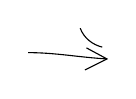
\begin{tikzpicture}[x=1cm,y=1cm,baseline=-.5ex]\draw (0,.08) .. controls (.35,.08) and (.65,.02) .. (1,0);\draw (.74,.14)--(1,0)--(.72,-.14);\draw (.66,.39) .. controls (.71,.26) and (.82,.18) .. (.94,.15);\end{tikzpicture}}C$ is surjective (in the passage cited) Now, since $u^{\unsure{o|0|\circ}}$ is injective, and $u^{\unsure{o|0|\circ}}=p^{\unsure{o|0|\circ}}\mathbin{o}v^{\unsure{o|0|\circ}}$, $v^{\unsure{o|0|\circ}}$ is also injective: it is an isomorphism, hence $v$ is an isomorphism, and, since $p$ is faithfully flat, the same is true of $u$.

\uline{Definitions \handwritten{11.15}}.- Given a field $k$, a $k$-vector space $V$, a $k$-group $G$ acting on $V$, and a vector $v\in V$, we say that $v$ is \uline{semi-invariant} under $G$ if the vector subspace $\handwritten{k.v}$ \deleted{be}\handwritten{is} stable under $G$.
\margin{\figure{\handwritten{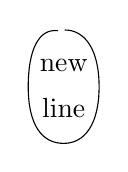
\begin{tikzpicture}[x=0.45cm,y=0.45cm]\draw (-.16,1.58) .. controls (-.7,1.65) and (-1,1.05) .. (-1,0) .. controls (-1,-1.1) and (-.6,-1.6) .. (0,-1.6) .. controls (.6,-1.6) and (1,-1.05) .. (1,0) .. controls (1,1.05) and (.6,1.6) .. (.03,1.6);\node at (0,0.6) {new};\node at (0,-0.6) {\unsure{line}};\end{tikzpicture}}}}
\figure{\handwritten{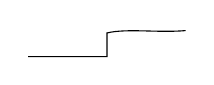
\begin{tikzpicture}[x=0.5cm,y=0.3cm]\draw (0,0) -- (2,0) -- (2,1) .. controls (2.5,1.2) and (3.3,1) .. (4,1.1);\end{tikzpicture}}}
Let $A$ denote the algebra of $G$, and $\handwritten{\rho}:V\handwritten{\longrightarrow}A\handwritten{\otimes}_k V$ the linear map which de-\linebreak fines the action of $G$ on $V$. To say that $v$ is semi-invariant under $G$ amounts to saying \deleted{that, for} that there exists $\handwritten{\lambda}\in A$ such that, for every $w\in kv$, $\handwritten{\rho}(w)=\handwritten{\lambda\otimes}w$. When $v\handwritten{\neq}0$, the element $\handwritten{\lambda\in}A$ is uniquely determined by this relation, we shall call it the \deleted{\uline{invariant}}\inserted{\handwritten{\uline{weight}}} of the semi-invariant element $\handwritten{v}$.

\deleted{On the other hand, $v$ is interpreted as an element of the bidual of $V$, hence as a section of $\handwritten{\unsure{\mathbb{V}|V}}(V)$; let $\handwritten{\varphi}:G\handwritten{\times\mathbb{V}}(V)\handwritten{\longrightarrow\mathbb{V}}(V)$ denote the morphism defining the action of $G$ on $\handwritten{\mathbb{V}}$.} To say that $v$ is semi-invariant \deleted{amounts to saying that there exists $\unsure{g\in k|\lambda\in k}$} with invariant $\handwritten{\lambda}$ amounts to saying that $\handwritten{\varphi}(g,v)=\handwritten{\unsure{\lambda|\widetilde{\lambda}|\chi}}(g)v$ for every $g\in G(k)$, where $\deleted{\handwritten{\unsure{\varphi:G\longrightarrow\underline{G}_{m,k}|\chi:G\longrightarrow\underline{G}_{m,k}}}}\inserted{\handwritten{\unsure{\lambda|\widetilde{\lambda}|\chi}:G\longrightarrow\underline{G}_{m,k}}}$ is the morphism defined by $\handwritten{\lambda}$. We thus see that $\handwritten{\lambda}$ \deleted{corresponds to}\inserted{\handwritten{is}} a character \deleted{\handwritten{\unsure{$\chi$}}} of $G$, called the \uline{associated character} of the semi-inva-\linebreak riant element $v$. \deleted{Finally we shall call the weight of the semi-invariant element $v$ the weight of the character $\handwritten{\chi}$ associated with $v$.}
\margin{\handwritten{!}}
